\section{Proof-of-Stake (PoS)\label{pos}}

\begin{otherlanguage}{english}\sloppy

Proof-of-Stake, josta tässä tutkielmassa käytetään lyhennettä PoS, sai alkunsa vastauksena PoW:n energiankulutukselle \cite{pos2}. PoS:n ideana on, että lohkoketjun konsensusmekanismi ei perustu laskennalliselle tehokkuudelle, vaan taloudilleselle haitalle mikä aiheutuu louhijoille mikäli lohkoketjua yritetään hyödyntää haitallisessa mielessä. Louhijoita PoS:sa kutsutaan usein osakkaiksi (stakers).

\vspace{1mm}

\begin{figure}[!htbp]
\centering
\fbox{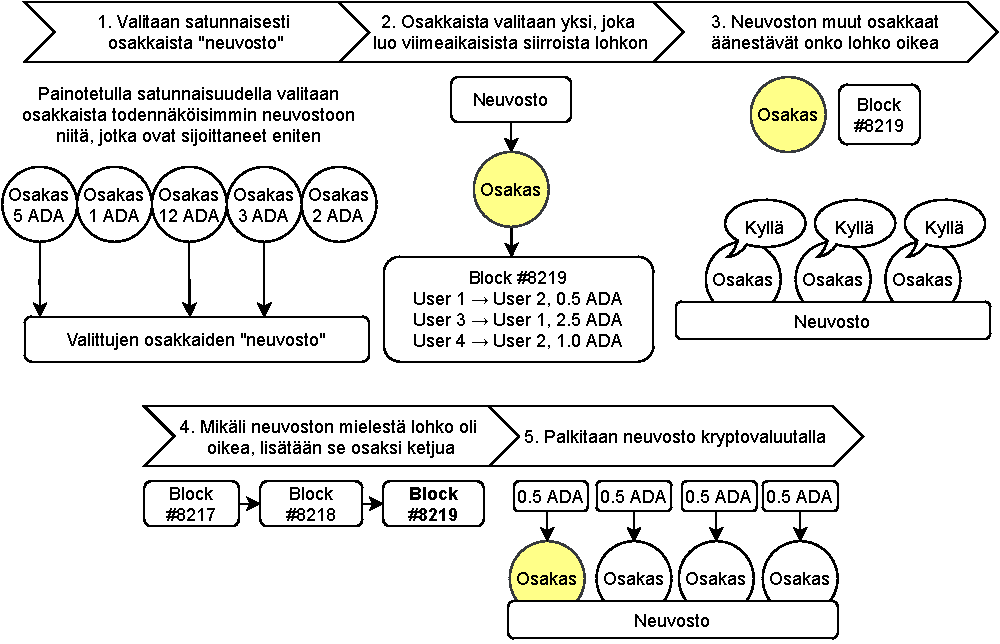
\includegraphics[width=0.98\textwidth]{proof-of-stake}}
\caption{Esimerkki Proof-of-Stake konsensusmekanismin toimintaperiaatteesta}
\label{fig_pos}
\end{figure}

\vspace{1mm}

PoS lohkoketjujen malli koostuu viidestä eri osasta \cite{pos1, pos2}:

\begin{enumerate}
\item Konsensus, missä jokin tietty osuus osakkaista (stakers) ovat yhteisymmärryksessä siitä, että lohkoketjuun tehdyt lisäykset ovat oikeita. Kuvaaja \ref{fig_pos} esittää esimerkin siitä, että konsensus voidaan saavuttaa valitsemalla osakkaista satunnaisella valinnalla neuvosto, joka äänestää uuden lohkon lisäämisestä lohkoketjuun.
\item Osakkuus, eli sijoittamisprosessi, missä käyttäjä voi ryhtyä osakkaaksi sijoittamalla jonkin määrän kryptovaluuttaa lohkoketjuun. Sijoitettu kryptovaluutta lukitaan tyypillisesti joksikin ennalta määrätyksi ajaksi, jolloin sijoitettuja varoja ei voi käyttää.
\item Palkitseminen, missä osakkaille jaetaan sijoitetun valuutan mukaan suhteutettu palkinto siitä, että he ovat olleet osallisina lohkoketjun turvaamisessa hyväksymällä uusia lohkoja. Kuvaaja \ref{fig_pos} esittää esimerkin siitä, miten palkkion saa neuvostoon valitut jäsenet, jotka olivat mukana lohkoketjun varmistamisessa.
\item Rankaiseminen, missä lohkoketjun väärinkäytöstä tai sen yritykseen syyllistyneiden käyttäjien lukitsemista varoista vähennetään jokin osuus. Rankaisuja tapahtuu myös joissakin tapauksissa myös silloin, mikäli osakas valitaan neuvostoon (ks. kuvaaja \ref{fig_pos}) ja jättää äänestämättä tai mikäli neuvostoon valittu osakas yrittää hyväksyä kahta lohkoa yhtäaikaisesti (double signing).
\item Uudelleenvalinta, missä valitaan tyypillisesti painotetun satunnaisuuden perusteella osakkaat, jotka hyväksyvät seuraavan lisäkysen lohkoketjuun. Myös muiden valintaperusteiden käyttö on mahdollista, mutta tyypillisesti valinta tapahtuu painotetulla satunnaisuudella, missä enemmän kryptovaluuttaa sijoittaneet osakkaat todennäköisemmin valikoituvat hyväksymään lisäyksiä lohkoketjuun.
\end{enumerate}

Proof-of-Stake konsensusmekanismin ollaan havaittu sen eri implementaatioissa olevan hyvin vähän energiaa kuluttava. Ongelmia kuitenkin on: matala yksityisyys, pääoman kasautuminen muutamalle osakkaalle ja skaalautuvuus nousevat usein esiin PoS:n kohdistuvassa kritiikissä. Näiden lisäksi lohkoketjujen sisältämää dataa ja infrastruktuuria ylläpitävien solmujen käyttämä laitteisto ja määrä vaikuttavat lohkoketjun sähkönkulutukseen. PoS:n energiankulutuksessa joudutaankin tyypillisesti tasapainottelemaan siinä, että halutaanko korkea hajautuneisuus suurella määrällä solmuja, vai pieni energiankulutus vähemmällä määrällä solmuja jolloin lohkoketjun hajautuneisuus on huonompi.

Seuraavaksi tutkielma esittelee kaksi Proof-of-Stake konsensusmekanismilla toimivaa lohkoketjua: Cardanon ja Algorandin. Cardano-lohkoketju ei ole vielä ottanut älysopimustoiminnallisuuksiaan käyttöön, mutta sen energiatehokkuudesta on jo laajalti tilastoja.

\subsection{Cardano\label{cardano}}
\begin{otherlanguage}{english}

Cardanon on kehittänyt Charles Hoskinsonin perustama IOHK vuonna 2015 \cite{cardanowhitepaper, iohk}, ja Cardanon sekä sen ekosysteemin kehitystä valvoo itsenäinen Cardano Foundation. 

Cardano käyttää PoS-protokollanaan viiden eri akateemisen instituution yhteistyössä kehittämää Ouroboros-lohkoketjuprotokollaa \cite{cardanowhitepaper}. Ouroboros on PoS-konsensusmekanismia soveltava lohkoketjuprotokolla \cite{cardano-ouroboros}, joka on kehitetty ratkaisuksi Bitcoinin korkeaan energiakulutukseen.

Cardanon tavoitteena on rakentua akateemisesti vertaisarvioitujen tutkimuksien pohjalta, ja sen Ourobos-protokolla mahdollistaa useiden eri ominaisuuksien implementoinnin modulaarisesti \cite{cardanowhitepaper}. Ourobos-protokolla mahdollistaa joustavan kehitysprosessin, jonka ansiosta Cardano lohkoketjuna on skaalattavampi ja tulevaisuudenkestävämpi. Cardanossa on erilaisia satunnaislukugeneraattoreita, mitkä ovat muissa lohkoketjuissa harvinaisia sekä mahdollisuus sivuketjuille (side-chains).

Cardanon käyttämä PoS-konsensusmekanismi on energiakulutukseltaan verrattuna PoW- konsensusmekanismeihin alhainen, sillä PoS ei tarvitse lainkaan laskennalliseen tehokkuuteen tai allokoidun tallennustilan suuruuteen perustuvaa todentamista \cite{cardanowhitepaper}. Cardanon energiakulutuksen on arvioitu 2021 olevan 6 gigawattituntia \cite{cardanoenergy}, missä yhden siirtoon vaadittu energiankulutus on keskimäärin 0.5479 kilowattituntia. Ouroboroksesta 2017 vuonna julkaistu tutkimus osoittaa, että Cardano kykeneen nykymuodossaan käsittelemään noin 257 siirtotapahtumaa sekunnissa \cite{cardano-tps}, mutta tämän oletetaan skaalautuvan satoihin tuhansiin mikäli Cardano implementoi niin kutsutun Hydra-menetelmän \cite{cardano-hydra}. Hydra-menetelmässä lohkoketjun siirtotapahtumia voidaan suorittaa päälohkoketjun lisäksi niin kutsutuissa layer-2 sivuketjuissa, joista kukin kykenee Hydra-menetelmän mukaan suorittamaan noin tuhat siirtotapahtumaa sekunnissa.

\end{otherlanguage}
\begin{subsection}{Algorand\label{algorand0}}
\begin{otherlanguage}{finnish}

Algorand-lohkoketjun kehittäjänä toimii Silvio Micalin vuonna 2017 perustama Algorand, Inc. yritys \cite{algorandwhitepaper}. Algorandin pääverkko julkaistiin 2019, ja lohkoketjuna se pyrkii toimimaan ympäristöystävällisesti hyödyntämällä Proof-of-Stake konsensusmekanismin mahdollistamaa energiatehokkuutta. Tämän lisäksi Algorandin tavoitteena on olla skaalautuva lohkoketju mahdollistaen kymmeniä tuhansia siirtotapahtumia sekunnissa.

Lamportin ja kollegoiden vuonna 1982 esittämässä tutkimuksessa \cite{byzantine} esitettiin hajautettuja järjestelmiä käsittelevä niin kutsuttu Bysantin kenraaliongelma. Algorand on pyrkinyt ratkaisemaan kyseisen ongelman, ja esittää Proof-of-Stake konsensusmekanismin ratkaisuksi kyseiseen ongelmaan \cite{algorandtech}. Bysantin kenraaliongelma on hyvä esimerkki kaikkien hajautettujen järjestelmien haasteesta, ja onkin hyvin sovellettavissa lohkoketjuihin: osa kenraaleista on pettureita ja osa luotettavia. Kenraaleiden täytyy pyrkiä valmistelemaan hyökkäys, ja mikäli valmistelun tehneet kenraalit ovat pettureita, saattaa päätös olla epäsuotuisa. Näin ollen täytyy pyrkiä saada konsensus luotettavien kenraaleiden kesken, vaikka on mahdotonta tietää ketkä kenraaleista on luotettavia.

Algorand käyttää algoritmista satunnaisuutta Proof-of-Stakessa \cite{algorandtech}. Kuka tahansa käyttäjistä voi sijoittaa valuuttaa (stake) lohkoketjuun, ja on tällöin Bysantin kenraaliongelmassa yksi kenraaleista. Algorand on skaalatuissa testeissä todennut, että mikäli 2/3 lohkoketjuun sijoitetuista varoista on luotettavien kenraalien hallussa, tulee tällöin sen käyttämällä painotetulla satunnaisella valinnalla valituksi luotettavat kenraalit. Painotettu satunnainen valinta Algorandissa toimii niin, että ne käyttäjät joilla on sijoitettuna enemmän varoja tulevat todennäköisemmin valituksi päätöksen tekeviksi kenraaleiksi.

Lohkoketjuissa kuitenkaan ei puhuta kenraaleista, vaan Algorandin tutkimuksissa esittämä kenraaliongelma vastaa Proof-of-Stake konsensusmekanismeissa tyypillistä uusien lohkojen hyväksyjien valintaa joka tehdään sijoitettuja varojen mukaan painotetulla satunnaisella valinnalla, kuten kuvaajassa \ref{fig_pos}. Cardano käyttää myös tällaista valintaperiaatetta \cite{cardanowhitepaper}.

Algorand sisältää myös Cardanon tapaan virtuaalikoneen (Algorand Virtual Machine, AVM), jolla on mahdollista ohjelmoida älysopimuksia ja applikaatioita, jotka hyödyntävät lohkoketjuja. Algorandin energiakulutus yhtä siirtoa kohden on varsin alhainen verratunna muihin lohkoketjuihin johtuen sen teknologian mahdollistamasta transaktiot-per-sekunti (TPS) määrästä: Algorand pystyy jo tällä hetkellä hyväksymään 1300 transaktiota sekunnissa, ja arvioi pystyvänsä tulevaisuudessa skaalaamaan määrän kymmeniin tuhansiin \cite{algorand-energy-2}. Algorand huhtikuussa 2021 arvioi kuluttaneensa vain 0,000008 kilowattituntia \cite{algorand-energy-2} yhtä siirtotapahtumaa kohden, kun taas Bitcoin kulutti samaan aikaan 930 kilowattituntia siirtoa kohden ja Ethereum 70 kilowattituntia. Arvioidulla energiankulutuksellaan siirtotapahtumaa kohden Algorand kuluttaisi keskimäärin vuodessa 4,9 gigawattituntia energiaa. Energiankulutus on kuitenkin mitattu Algorandin kehitystiimin toimesta käyttäen laskennassa ainoastaan optimaalisinta laitteistoa (Raspberry Pi 4), minkä vuoksi todellinen energiankulutus on mahdollisesti huomattavasti suurempi. Tämän lisäksi Algorandin asettamat minimilaitesuositukset solmun ylläpitämiselle eivät vastaa laskelmissa käytettyä Raspberry Pi 4:sta, sillä minimilaitesuositukset vaativat solmulta viidensadan gigatavun NVMe SSD:n \cite{algorand-min-specs} mitä Raspberry Pi 4:sta ei löydy. Laskelmat on myös tehty oletuksella, että lohkoketju käsittelisi sen maksimäärän verran transaktioita sekunnissa, eli 1300 joka sekunti, vaikka Algorand on vuonna 2021 keskimäärin toiminut alle kymmenesosalla tästä luvusta \cite{algorand-explorer}.

Plattin ja kollegoiden syyskuussa 2021 julkaisemassa tutkimuksessa \cite{algorand-energy} tehtiin arvio Algorandin energiankulutuksesta käyttämällä laskennassa realistisempaa laitteistoa ja sen siirtotapahtumien oikeaa määrää teoreettisen maksimikapasiteetin sijaan. Tällöin laskennassa saavutettiin tulokseksi 0,00534 \cite{algorand-energy} kilowattituntia per transaktio. Plattin ja kollegoiden tutkimus laski, että Algorand suorittaa todellisuudessa keskimäärin 9,85 \cite{algorand-energy} siirtotapahtumaa sekunnissa. Tällöin Algorandin vuosittainen energiankulutus on noin 1,684 gigawattituntia. Tutkielma käyttää tätä lukua vertailussa, sillä aikaisemmin mainituista syistä Algorandin kehittäjätiimin oma arvio on epärealistinen ja kehittäjätiimin oma tutkimus ei ole puolueeton. 

\end{otherlanguage}
\end{subsection}


\end{otherlanguage}